% das Papierformat zuerst
\documentclass[a4paper, 11pt]{article}
\usepackage[margin=3cm]{geometry}
\usepackage[utf8]{inputenc}
\usepackage[T1]{fontenc}
\usepackage[fleqn]{amsmath} %left aligned equations
\usepackage{hyperref} % clickable refs
\usepackage{graphicx}
\usepackage[toc, numberedsection]{glossaries}
\usepackage{float}
\usepackage{amssymb}
\usepackage{calc}
\usepackage{enumitem} 
\usepackage{url}
\usepackage{parskip}
% http://tex.stackexchange.com/questions/17730/newcommand-and-spacing
\usepackage{xspace}

% TODO: template übersetzten

\makeglossaries

%Hack for referencing labels
\makeatletter
\def\namedlabel#1#2{\begingroup
    #2%
    \def\@currentlabel{#2}%
    \phantomsection\label{#1}\endgroup
}
\makeatother
% End: Hack for referencing labels

% Glossar: alle Einträge, aber ohne extra Referenzen
% http://tex.stackexchange.com/questions/115635/glossaries-suppress-pages-when-using-glsaddall
\newcommand*{\glsgobblenumber}[1]{}
\makeatletter
\newcommand*{\glsaddnp}[2][]{
  \glsdoifexists{#2}{
    \def\@glsnumberformat{glsgobblenumber}
    \edef\@gls@counter{\csname glo@#2@counter\endcsname}
    \setkeys{glossadd}{#1}
    \@gls@saveentrycounter
    \@do@wrglossary{#2}
  }
}
\renewcommand{\glsaddallunused}[1][]{
  \edef\@glo@type{\@glo@types}
  \setkeys{glossadd}{#1}
  \forallglsentries[\@glo@type]{\@glo@entry}{
    \ifglsused{\@glo@entry}{}{
      \glsaddnp[#1]{\@glo@entry}}}
}
\makeatother

\renewcommand{\glsnamefont}[1]{\mdseries #1} % glossary entries shouldn’t be bold

% Glossar

% So sieht ein Glossar-Eintrag aus:
%
%\newglossaryentry{dijkstra}{
%  name={Dijkstra’s Algorithmus},
%  description={ein Algorithmus, um den optimalen Pfad in einem gerichteten Graphen zu finden}
%}
%\newglossaryentry{arc}{
%  name={Arc-Flags},
%  description={eine Technik, um Routenberechnung zu beschleunigen},
%  see={dijkstra}
%}
%
% Und so kann er im Dokument verwendet werden:
%
% lorem ipsum dolor sit \gls{arc}, consectetur
%
% End: Glossar

% usage: \counteditem{prefix}{refName} -> item `/prefixXX/` with label `prefix:refName` (where XX is counted in increments of 10)
\makeatletter
\newcommand{\oitem}[2]{
  % define the counter
  \@ifundefined{c@oitem#1}{\newcounter{oitem#1}}{} % initialized at 0
  \addtocounter{oitem#1}{10}
  \item[\namedlabel{#1:#2}{/#1\arabic{oitem#1}/}]
}
\makeatother

% usage: \testfall{szenario}{ablauf}{ergebnis} oder \testfall[\ref{F:getesteteFunktion}]{szenario}{ablauf}{ergebnis}
\newcommand{\testfall}[4][]{
  \begin{description}
    \ifthenelse{\equal{#1}{}}
               {} % optional argument #1 is empty: skip
               {\item[Testet] #1}
    \item[Vorbedingungen] #2
    \item[Ablauf] #3
    \item[Erwartetes Ergebnis] #4
  \end{description}
}

\newcommand{\testsequence}[3][]{
	\begin{description}[leftmargin=!,labelwidth=\widthof{\bfseries Preconditions}]
		\ifthenelse{\equal{#1}{}}
		{} % optional argument #1 is empty: skip
		{\item[Tests] #1}
		\item[Preconditions] #2
		\item[Steps] #3
	\end{description}
}

\begin{document}

% place a symbol before clickable links
% this has to come *after* \begin{document} because hyperref installs a \AtBeginDocument hook that updates the ref command.
\newcommand{\refsymbol}[0]{\scalebox{0.5}{$\nearrow$}}
\let\oldref\ref
\renewcommand{\ref}[1]{\refsymbol\oldref{#1}}
\let\oldgls\gls
\renewcommand{\gls}[1]{\refsymbol\oldgls{#1}}
\let\oldGls\Gls
\renewcommand{\Gls}[1]{\refsymbol\oldGls{#1}}
\let\oldglspl\glspl
\renewcommand{\glspl}[1]{\refsymbol\oldglspl{#1}}
\let\oldGlspl\Glspl
\renewcommand{\Glspl}[1]{\refsymbol\oldGlspl{#1}}
\let\oldglslink\glslink
\renewcommand{\glslink}[2]{\refsymbol\oldglslink{#1}{#2}}
\let\oldhyperref\hyperref
\renewcommand{\hyperref}[2][notActuallyOptional]{\refsymbol\oldhyperref[#1]{#2}}
\let\oldautoref\autoref
\renewcommand{\autoref}[1]{\refsymbol\oldautoref{#1}}

\newcommand{\abbildung}[1]{\autoref{fig:#1}}
\newcommand{\mamid}{\textit{MAMID}\xspace}

% alle Glossareintraege
\newacronym{gui}{GUI}{Graphical User Interface}
\newacronym{cli}{CLI}{Command Line Interface}
\newacronym{CRUD}{CRUD}{Create / Read / (Update|Modify) / Delete}
\newacronym{ICMP}{ICMP}{Internet Control Message Protocol}
\newacronym{API}{API}{Application Programming Interface}
\newacronym{JSON}{JSON}{JavaScript Object Notation}
\newacronym{HTTP}{HTTP}{HyperText Transfer Protocol}
\newacronym{LAN}{LAN}{Local Area Network}
\newacronym{WAN}{WAN}{Wide Area Network}

\newglossaryentry{cluster}{
	name={cluster},
	description={Aggregation of \glspl{host}},
	plural={clusters}
}
\newglossaryentry{MongoDB}{
	name={MongoDB},
	description={A NoSQL based database server},
	plural={MongoDB}
}
\newglossaryentry{replica set}{
	name={replica set},
	description={Multiple \gls{MongoDB} instances distributed over multiple \glspl{host} sharing a copy of the same data},
	plural={replica sets}
}
\newglossaryentry{sharding}{
	name={Sharding},
	description={A type of \gls{MongoDB} deployment where data sets are spread across multiple \glspl{host} or \glspl{replica set}. \\ More information: {\small \url{https://docs.mongodb.com/manual/sharding/}}}
}
\newglossaryentry{administrator}{
	name={administrator},
	description={The person responsible for managing the hardware \& software deployed on the \gls{cluster}. Uses \mamid for \gls{MongoDB} \gls{replica set} administration},
	plural={administrators}
}
\newglossaryentry{host}{
	name={host},
	description={Network node with a unique hostname},
	plural={hosts}
}
\newglossaryentry{slave}{
	name={slave},
	description={Program running on \gls{host} managing \gls{MongoDB} processes},
	plural={slaves}
}
\newglossaryentry{master}{
	name={master},
	description={Program responsible for managing \glspl{slave} and providing \acrshort{API} for \gls{cluster} management},
	plural={masters}
}
\newglossaryentry{inventory}{
	name={inventory},
	description={Persistently stored list of slaves and their state (see \ref{D:Inventory})},
	plural={inventories}
}
\newglossaryentry{active mode}{
	name={active mode},
	description={Marks the \gls{slave} as available to host \gls{MongoDB} processes that are be part of \glspl{replica set}.},
	plural={active modes}
}
\newglossaryentry{maintenance mode}{
	name={maintenance mode},
	description={Marks the \gls{slave} as unavailable \& inhibits reconfiguration through \gls{master}, but does not otherwise affect running \gls{MongoDB} instances on the \gls{host}.},
	plural={maintenance modes}
}
\newglossaryentry{disabled mode}{
	name={disabled mode},
	description={A \gls{slave} in this mode does not run any \gls{MongoDB} instances controlled by the \gls{master}, hence has no \gls{MongoDB} instances in any \gls{replica set}.},
	plural={disabled modes}
}
\newglossaryentry{risk group}{
	name={risk group},
	description={A set of \glspl{host} sharing a common risk of failure, e.g. a shared power supply. Modeled through sets of \glspl{slave} since a 1:1 relationship exists between hosts and slaves},
	plural={risk groups}
}
\newglossaryentry{persistent storage}{
	name={persistent storage},
	description={Storage capable of storing data between power outage},
	plural={persistent storages}
}
\newglossaryentry{volatile storage}{
	name={volatile storage},
	description={Storage incapable of storing data between process lifetime},
	plural={volatile storages}
}
\newglossaryentry{root data directory}{
	name={root data directory},
	description={Base directory holding all files of a \gls{slave} and its \gls{MongoDB} instances},
	plural={root data directories}
}
\newglossaryentry{arbiter}{
	name={arbiter},
	description={In charge of breaking ties on a \gls{replica set} election with even number of members. More information: {\small \url{https://docs.mongodb.com/manual/core/replica-set-elections/}}},
	plural={arbiters}
}
\newglossaryentry{degraded}{
	name={degraded},
	description={State of a \gls{replica set} with member in \gls{maintenance mode} or \gls{disabled mode} or otherwise reporting failure},
	plural={degraded}
}

\begin{titlepage}
\makeatletter
\begin{center}
~\\[4em]
{\Huge MAMID}\\[.8em]\huge{Monitor and Manager for In-Memory Databases}\\[2em]
{\huge Functional specification}\\[1em]
{\large\today}\\[2.5em]
{\LARGE
Niklas Fuhrberg\\
Anton Schirg\\
Christian Schwarz\\
Janis Streib\\
Bob Weinand\\[3em]}
supervised by\\[2em]
{\Large
Dr. Marek Szuba\\[1em]}
at\\[1em]
{\Large
Karlsruhe Institute of Technology\\
SCC}

\end{center}
\makeatother
\end{titlepage}
\newpage
\tableofcontents
\newpage

% -------------------------------------------------------------- HIER BEGINNT DAS DOKUMENT WIRKLICH ---------------------------------
\section{Introduction}
\mamid is a manager for database \glspl{cluster}, facilitating creation, administration and monitoring of \gls{MongoDB} \glspl{replica set}.

\mamid assists the \gls{administrator} during initial setup, continuous operation, maintenance cases and expansion of the cluster.

The \gls{administrator} describes the \gls{cluster} \glspl{host} and the desired \gls{MongoDB} \glspl{replica set}.

Each \gls{host} runs a \gls{slave} application of \mamid, allowing control of the \glspl{host} from a single \gls{master} instance of \mamid.

\mamid utilizes the \gls{administrator}'s description of the cluster and replica sets to run \gls{MongoDB} instances on the \glspl{host}.

\mamid configures the \gls{MongoDB} instances to form the desired replica sets.

\mamid monitors the deployed configuration continuously and informs the \gls{administrator} about problems (when they arise).

Maintenance of individual \glspl{host}, growing \& shrinking of the cluster, etc. is announced to \mamid beforehand, allowing for reconfiguration of the deployed \glspl{replica set} if necessary.

A possible deployment of \mamid is depicted in Figure \ref{fig:cluster_layout}.

\begin{figure}[H]
	\centering
	\includegraphics[width=\textwidth]{cluster_layout}
	\caption{Possible cluster layout for a single application built on MongoDB}
	\label{fig:cluster_layout}
\end{figure}

\section{Objectives \& Criteria}
\subsection{Must-Have Criteria}

\subsubsection{Cluster Description by Administrator}
% TODO analyze whether the given criteria can be phrased more abstractly \& move the details to (new) functional requirements. (-> forward lookup references from criteria to functional requirement if required)
\begin{description}

\oitem{MK}{} The \gls{administrator} interacts with \mamid through a web \acrshort{gui}.

% inventory ops
\oitem{MK}{inventory_definition} The \gls{master} maintains a list of \glspl{slave} called \gls{inventory}.
\begin{description}
\oitem{MK}{} The \acrshort{gui} visualizes the \gls{inventory}.
\oitem{MK}{} The \gls{administrator} can add \glspl{slave} to the \gls{inventory}.
\oitem{MK}{} The \gls{administrator} can remove a \gls{slave} that does not host any \gls{MongoDB} processes from the \gls{inventory}.
\oitem{MK}{spec_risk_groups} The \gls{administrator} can model a shared risk of failure between \glspl{host}, e.g. a shared power supply.
\oitem{MK}{available_slave_types} The \gls{administrator} can specify whether the \gls{slave} has \glslink{persistent storage}{persistent (typically HDD/SSD backed)} or \glslink{volatile storage}{volatile (RAM backed)} storage.
\oitem{MK}{root_data_directory} The \gls{administrator} can specify in which filesystem directory on the \gls{host} the \gls{slave} and its \gls{MongoDB} processes store data.
% inventory ops -> slave
\oitem{MK}{slave_mode_active} The \gls{administrator} can announce to \mamid that a slave is ready to host MongoDB processes.
\oitem{MK}{slave_mode_maintenance} The \gls{administrator} can announce to \mamid that a slave is in maintenance to inhibit automatic reconfiguration of its MongoDB processes.
\oitem{MK}{slave_mode_disabled} The \gls{administrator} can announce to \mamid that a slave should not host any MongoDB processes.
\end{description}

% replica set ops
\oitem{MK}{replica_set_create} The \gls{administrator} can describe a new \gls{MongoDB} \gls{replica set} by specifying constraints on how it should be configured by \mamid.
\begin{description}
\oitem{MK}{replica_set_config_profiles} The \gls{administrator} can --- on creation of a replica set (\ref{MK:replica_set_create}) --- specify that it must be usable as a configuration server for \gls{MongoDB} \gls{sharding}.
\oitem{MK}{replica_set_member_total_counts} The \gls{administrator} can select the number of \gls{MongoDB} instances (members) of a replica set.
\oitem{MK}{replica_set_member_pv_counts} Volatile and persistent member count of a \gls{replica set} can be independently configured, under constraints described in \ref{F:master_alloc_resp_pv_counts}.
\end{description}
\oitem{MK}{} The \acrshort{gui} visualizes the list of configured \glspl{replica set}.
\oitem{MK}{} The \gls{administrator} can destroy a \gls{replica set}.

\end{description}

\subsubsection{MongoDB Configuration \& Monitoring}
\begin{description}
\oitem{MK}{mongod_deployment1} \mamid asserts that the replica sets described by the administrator are configured on the cluster (see \ref{MK:replica_set_create}).
\oitem{MK}{mongod_deployment2} To achieve \ref{MK:mongod_deployment1}, \mamid spawns \& controls \gls{MongoDB} processes on the hosts using a \gls{slave} process.
\begin{description}
	\oitem{MK}{mongod_redeployment} \mamid redeploys configured \gls{MongoDB} processes to hosts where the \gls{slave} process reports a situation different from what is expected by the \gls{master}.
	\oitem{MK}{mongod_redeployment_powercycle_specific} Specifically, a host with volatile data storage can loose all data originating from the \gls{slave} process or \gls{MongoDB} and is automatically redeployed with correctly configured \gls{MongoDB} instances (\ref{MK:mongod_deployment2}).
\end{description}
% Todo old \oitem{MK}{} The \gls{master} deploys the \gls{replica set} configuration described by the administrator to the cluster.

% monitoring features
\oitem{MK}{detect_slave_unexpected_behavior} \mamid detects when a \gls{slave} in the \gls{inventory} behaves unexpectedly, e.g. when it becomes unreachable and the administrator did not announce maintenance to \mamid beforehand.
\oitem{MK}{} \mamid informs the \gls{administrator} by e-mail about problems in the cluster (\ref{MK:detect_slave_unexpected_behavior}).
\oitem{MK}{} The \acrshort{gui} visualizes \glspl{slave} behaving unexpectedly (\ref{MK:detect_slave_unexpected_behavior}).
\end{description}

\subsection{Optional Criteria}
\begin{description}
	
% master
\oitem{WK}{api_authentication} \mamid requires authentication for administrative actions.
	
% inventory
\oitem{WK}{manual_autodiscovery} \mamid auto-discovers new \glspl{slave} on the \gls{administrator}'s request.
\oitem{WK}{continuous_autodiscovery} \mamid continuously auto-discovers new \glspl{slave}.
\oitem{WK}{monitor_icmp} \mamid recognizes when the \gls{slave} software does not respond but the corresponding \gls{host} is still connected to the network.
\oitem{WK}{export_import_snapshot} The \gls{administrator} can backup and restore the cluster description.

% slaves
\oitem{WK}{tweak_performance_parameters} The \gls{administrator} can customize performance-relevant parameters of \gls{MongoDB} processes.

% automatic repair
\oitem{WK}{auto_repair} \mamid supports automatic reconfiguration when detecting unexpected behavior of \glspl{slave}. The failing slave is marked as unsuitable to host \gls{MongoDB} processes and redeployment is triggered to repair the degraded replica sets (extends \ref{MK:detect_slave_unexpected_behavior}).

% replica sets
\oitem{WK}{deploy_arbiters} The \gls{master} deploys \gls{MongoDB} \glspl{arbiter} for configured \glspl{replica set}, removing some restrictions in \ref{F:master_alloc_resp_pv_counts}.
\oitem{WK}{} The \gls{master} exposes machine metrics of the \glspl{slave}.
\oitem{WK}{} The \gls{master} exposes the \glspl{replica set}' replication status.

% other
\oitem{WK}{} The \gls{administrator} can interact with \mamid via a \acrshort{cli}.
\oitem{WK}{http_api} The \gls{administrator} can interact with \mamid via a stable, documented \acrshort{HTTP} \acrshort{API}.
\end{description}

\subsection{Demarcation Criteria}
\begin{description}
\oitem{AK}{} The \gls{administrator} does not directly configure individual \gls{MongoDB} instances spawned \& controller by \mamid. All configuration happens through \mamid, either automatically (e.g. replica set deployment) or through a \mamid interface (e.g. GUI, CLI, HTTP API).
\oitem{AK}{} The \gls{master} does not implement support for higher-layer \gls{MongoDB} features, e.g. \gls{sharding}.
\oitem{AK}{} \mamid neither deploys the operating system nor other required software (such as \gls{MongoDB} binaries) to the \gls{cluster} \glspl{host}.
\end{description}

\section{Product Usage}

\subsection{Scope of Application}
\begin{itemize}
\item \gls{MongoDB} \glslink{cluster}{Cluster} Administration
\item High-Availibility MongoDB Deployment
\item MongoDB Cluster Monitoring
\end{itemize}

\subsection{Target Users}
\begin{itemize}
\item Cluster \glspl{administrator} in charge of creating a MongoDB replica set deployment.
\end{itemize}

\subsection{Operating Conditions}
\begin{itemize}

\item Low maintenance capacity for the cluster (time, personnel)
\item Uncomplicated takeover by a successor must be possible (flat learning curve)
\end{itemize}

\section{Operational Environment}

\begin{figure}[H]
	\centering
	\includegraphics[width=\textwidth]{hardware_layout}
	\caption{Possible cluster hardware layout}
\end{figure}

\subsection{Software}\label{subsec:Software}
\begin{itemize}
\item Primary Target Operating System: Open Indiana Build 151a9 (Illumos Kernel, 64bit)
\item MongoDB version 3.2
\end{itemize}

\subsection{Hardware}
Each of the subsequently listed requirements is an extension of the previous one.
\subsubsection{Cluster Hosts: Hardware}
\begin{itemize}
	\item 64bit amd64 Instruction Set
	\item Up to $1GB$ file storage for \mamid applications.
	\item Sufficient \glslink{persistent storage}{persistent} or \gls{volatile storage} to hold the required \gls{MongoDB} data. \\
	\begin{itemize}
		\item \textbf{Note}: fewer \glspl{host} with \gls{persistent storage} may require the \gls{persistent storage} on these \glspl{host} to be larger.
	\end{itemize}
\end{itemize}

\subsubsection{Cluster Hosts: Interconnect}
\begin{itemize}
	\item All hosts are interconnected through fast \acrshort{LAN}.
	\begin{itemize}
		\item All cluster hosts are interconnected through an isolated \acrshort{LAN}
		\item $>= 1$ cluster host is connected to both the isolated \acrshort{LAN} and an external network (usually another \acrshort{LAN} or \acrshort{WAN}).
	\end{itemize}
\end{itemize}

\subsubsection{Operation of Persistently Stored Replica Sets}
\begin{itemize}
	\item $>= 1$ cluster host with \gls{persistent storage}
	\item $>= 3$ cluster hosts in total
\end{itemize}

\subsubsection{Basic Level of Host Redundancy}
\begin{itemize}
	\item $>= 3$ mutually disjoint sets of \gls{cluster} \glspl{host} that can be classified as not sharing a common risk of failure (see \ref{F:master_alloc_resp_risk_groups}).
\end{itemize}

\section{System Model}
\begin{figure}[H]
\includegraphics[width=\textwidth]{module_overview}
\caption{\mamid Modules Overview}
\end{figure}
\subsection{Master}\label{SM:Master}
\begin{description}
	\oitem{SM}{masterapiserver} Master::APIServer\\
	Provides an \acrshort{API} for \gls{cluster} status reporting and administrative activity. (\ref{F:master_api_crud_slaves}, \ref{F:master_api_crud_risk_groups}, \ref{F:master_api_set_slave_mode}, \ref{F:master_api_crud_repl_set_config}, \ref{F:master_api_error_reports}, \ref{WF:master_api_get_auto_discovered_slaves}, \ref{WF:master_api_machine_metrics}, \ref{WF:master_api_repl_set_status})
 	\oitem{SM}{} Master::Controller\\
	Controls flow of events between different \gls{master} submodules.\\
	Updates the inventory database (\ref{SM:inventory}) as state change is recognized by the monitor.\\
	Implements automatic administration as explained in \ref{WF:master_controller_auto_repair}.)
	\oitem{SM}{inventory} Master::Inventory\\
	Database containing
	\begin{itemize}
		\item list of \glspl{slave} and associated state
		\item list of configured \glspl{replica set}.
	\end{itemize}
	(\ref{F:master_inventory_persist_conf_state})
	\oitem{SM}{master_clusterallocator} Master::ClusterAllocator\\
	It lays out the \gls{cluster}, i.e. decides the distribution of mongod instances onto \gls{cluster} \glspl{host}. (\ref{F:layout_cluster_config})\\
	It respects constraints as described by \ref{F:master_alloc_resp_risk_groups}, \ref{F:master_alloc_resp_pv_counts}, \ref{F:master_alloc_resp_mode} and \ref{WF:master_alloc_arbiters}.\\
	It communicates with the \glspl{slave} using \ref{SM:masterslaveproto} to enforce the \gls{cluster} layout. (\ref{F:master_alloc_communicate_config})
	\oitem{SM}{master_monitor} Master::Monitor\\
	Is responsible for observing whether \glspl{slave} are still alive using \ref{SM:masterslaveproto} and auto-discovery. (\ref{F:master_monitor_config}, \ref{WF:master_monitor_icmp}, \ref{WF:master_monitor_continuous_auto_discovery})
\end{description}
\subsection{MasterSlaveProtocol}\label{SM:MasterSlaveProtocol}
\begin{description}
	\oitem{SM}{masterslaveproto} MasterSlaveProtocol\\
	Is responsible for communication between \gls{master} and \gls{slave}. (\ref{F:msp_trans_config}, \ref{F:msp_trans_reachability}, \ref{WF:msp_trans_mach_metr}, \ref{WF:msp_trans_repl_status})
\end{description}
\subsection{Slave}\label{SM:Slave}
\begin{description}
	\oitem{SM}{} Slave::Controller\\
	Dispatches instructions to the \glspl{MongoDB} client and the process manager. (\ref{F:slave_enforce_config})\\
	It notifies via \ref{SM:masterslaveproto} whether operations failed or succeeded as well as not locally recoverable failures. (\ref{F:slave_report_config}, \ref{WF:slave_report_machine_metrics}, \ref{WF:slave_report_repl_status})
	\oitem{SM}{mongodbclient} Slave::MongoDBClient\\
	Implements communication with \gls{MongoDB} processes. (\ref{F:slave_communicate_with_mongodb})
	\oitem{SM}{} Slave::ProcessManager\\
	Spawns and controls \gls{MongoDB} processes. (\ref{F:slave_control_procs})
\end{description}
\subsubsection{Slave Modes}\label{SM:SlaveModes}
\begin{figure}[H]
\centering
\includegraphics[width=\textwidth]{state_diagram}
\caption{Slave State Diagram}
\end{figure}
A slave can be in the following states:
\begin{itemize}
	\item \glslink{active mode}{active}\\
	\mamid monitors \glspl{slave} in active mode. \glslink{slave}{Slaves} in this mode behave as expected, i.e. are running MongoDB processes in the configuration determined by the \hyperref[SM:Master]{Master}.\\
	If the slave behaves unexpectedly, e.g. is not reachable, \mamid notifies the \gls{administrator} and sets its state to \emph{unknown}.
	\item \emph{unknown}\\
	\mamid monitors \glspl{slave} in \emph{unknown} state and sets them back to \gls{active mode} when they recover.\\
	\mamid can recover a slave in \emph{unknown} state automatically by respawning and configuring MongoDB processes, e.g. after power-loss on a \glslink{volatile storage}{volatile} \gls{host}.
	The \gls{administrator} can set the slave state
	\begin{itemize}
		\item to \gls{maintenance mode} to stop monitoring of the slave or
		\item to \gls{disabled mode} to trigger reallocation of all \gls{MongoDB} processes to another slave.
	\end{itemize}
	\item \glslink{maintenance mode}{maintenance}\\
	\mamid ignores unexpected slave behavior if the slave is in maintenance mode.\\The running MongoDB processes on the slave are not modified / reconfigured and no reallocation to other slaves is triggered.
	\item \glslink{disabled mode}{disabled}\\
	A \gls{slave} in disabled mode does not run any \gls{MongoDB} process controlled by the slave process. When a \gls{slave} with MongoDB processes in a \gls{replica set} is set to disabled mode, \mamid stops all these processes and configures new ones on other \glspl{slave} to repair the temporarily degraded replica set.
\end{itemize}
Slave state is tracked exclusively in the \hyperref[SM:Master]{Master}.\\
All state changes apart from active $\leftrightarrow$ unknown are triggered by the \gls{administrator}.\\
If \ref{WK:deploy_arbiters} is implemented the state change unknown $\rightarrow$ disabled can be triggered automatically.

\subsection{Graphical User Interface (GUI)}\label{SM:GUI}
\begin{description}
	%React-JS und so...
	\oitem{SM}{gui_model} GUI::Model\\
	Data structures representing \mamid entities that are displayed or managed through the web interface (\ref{SM:gui_view}). (\ref{F:gui_crud_inventory}, \ref{F:gui_set_slave_type}, \ref{F:gui_set_root_data_dir}, \ref{F:gui_set_risk_groups}, \ref{F:gui_set_slave_mode}, \ref{F:gui_crud_replica_sets})
	\oitem{SM}{gui_view} GUI::View\\
	Web interface and its UI elements. (\ref{F:gui_crud_inventory}, \ref{F:gui_crud_replica_sets}, \ref{F:gui_display_errors}, \ref{WF:gui_display_machine_metrics}, \ref{WF:gui_display_repl_status}, \ref{WF:gui_auto_discovery_interface})
	\oitem{SM}{} GUI::Controller\\
	Handles UI interaction, updates model and asserts semantic consistency between \ref{SM:gui_view} and \ref{SM:gui_model}.
\end{description}
\subsection{NotificationManager}\label{SM:NotificationManager}
\begin{description}
	\oitem{SM}{notif_mail} NotificationManager::MailNotifier\\
	Sends e-mail messages. (\ref{F:notifmgr_send_emails})
	\oitem{SM}{notif_apiclient} NotificationManager::APIClient\\
	\acrshort{API} client for \ref{SM:masterapiserver}. (\ref{F:notifmgr_consume_errors})
	\oitem{SM}{notif_controller} NotificationManager::Controller\\
	Uses \ref{SM:notif_apiclient} and \ref{SM:notif_mail} to implement notification of the \glspl{administrator}. (\ref{F:notifmgr_controller_send_errors}, \ref{F:notifmgr_read_conf_file})
\end{description}

\section{Product Data}

\subsection{Inventory (contains slaves)}\label{D:Inventory}
% hostname(PRIMARY KEY) | slaveport | mongod-portrange | persistent/volatile | root data directory | mode (active, maint, disabled)

List of tuples containing the following data

\begin{description}
	\oitem{D}{} hostname
	\oitem{D}{} \gls{slave} port $\in \mathbb{N}$
	\oitem{D}{slave_mongod_portrange} mongod-portrange $\in \{{[i, j]} \mid i,j \in \mathbb{N}\}$ (also specifies how many mongod instances may run on the slave)
	\oitem{D}{} persistency $\in \{\text{\glslink{persistent storage}{persistent}}, \text{\glslink{volatile storage}{volatile}}\}$
	\oitem{D}{} \gls{root data directory}
	\oitem{D}{} mode $\in \{\text{\glslink{active mode}{active}}, \text{\glslink{maintenance mode}{maintenance}}, \text{\glslink{disabled mode}{disabled}}\}$
\end{description}

\subsection{Replica Set Configuration}
%----------------------------- ADMIN SETTABLE ------------------------------------------------------------  ---Allocator settable--  
% replset | p = num of persistent slaves | v = num of volatile slaves | sharding config server (true|false) | p+v mongod processes 
List of tuples containing the following data

\begin{description}
	\oitem{D}{} \gls{replica set} name
	\oitem{D}{} number of \glslink{persistent storage}{persistent} slaves $p$
	\oitem{D}{} number of \glslink{volatile storage}{volatile} slaves $v$
	\oitem{D}{} \gls{sharding} configuration server $\in \{\text{true}, \text{false}\}$
	\oitem{D}{} member mongod processes (list of $p+v$)
\end{description}

\subsection{MongoDB processes}
%(hostname | port != slaveport) PRIMARY KEY
List of tuples containing the following data

\begin{description}
	\oitem{D}{} hostname
	\oitem{D}{} port
\end{description}

\subsection{Risk Groups}
\begin{description}
	\oitem{D}{} Mutually disjoint sets of \glspl{slave}. Membership of two \glspl{slave} in the same set denotes a shared risk of failure.
\end{description}

\section{Product Data Consistencies}

\begin{description}
	%Ports
	\oitem{DC}{} The port of a mongod process must be inside the mongod-portrange of the slave it is running on
	\oitem{DC}{} The combination of mongod hostname and mongod port must be unique
	\oitem{DC}{} The slave port must not be inside the mongod-portrange
	%Arbiters
	\oitem{DC}{} The number of nodes $p+v$ in a replica set must be odd unless \ref{WK:deploy_arbiters} is implemented
\end{description}


\section{Functional Requirements}
% Format: Substantiviertes Verb am Anfang („Bestimmen von X“, nicht „Bestimmung von X“, „Bestimme X“ oder „X bestimmen”).

%TODO cli paramters + config file template wf spezifizieren

\subsection{Graphical User Interface (GUI)}
The \acrshort{gui} acts as a frontend to the functionality provided by \ref{SM:masterapiserver}. Hence, all functionality described in this subsection is realized through \acrshort{API} calls to the \gls{master}.
\begin{description}
	\oitem{F}{gui_crud_inventory} \acrshort{CRUD} \glspl{slave} in \gls{inventory}.
	\oitem{F}{gui_set_slave_type} Specify type of \gls{slave} (\ref{MK:available_slave_types}) upon insertion into \gls{inventory}.
	\oitem{F}{gui_set_root_data_dir} Specify \gls{root data directory} of \glspl{slave} (\ref{MK:root_data_directory}).
	\oitem{F}{gui_set_risk_groups} \acrshort{CRUD} \glspl{risk group} (\ref{MK:spec_risk_groups}).
	\oitem{F}{gui_set_slave_mode} Set mode of \gls{host} to \glslink{active mode}{active}, \glslink{maintenance mode}{maintenance} or \glslink{disabled mode}{disabled}.
	\oitem{F}{gui_crud_replica_sets} \acrshort{CRUD} \gls{replica set} configurations (\ref{MK:replica_set_create}).
	\oitem{F}{gui_display_errors} Display error reports (\ref{F:master_api_error_reports}).
	\oitem{WF}{gui_display_machine_metrics} Display machine metrics of the \glspl{slave}. 
	\oitem{WF}{gui_display_repl_status} Display replication status of the configured \glspl{replica set}.
	\oitem{WF}{gui_auto_discovery_interface} Provide interface to select auto-discovered \glspl{slave} when adding to \gls{inventory} (\ref{F:gui_crud_inventory}).
	\oitem{WF}{gui_command_line_parameters_interface} Provide interface to specify command line parameters for \gls{MongoDB} processes (\ref{WK:tweak_performance_parameters}).
\end{description}

\subsection{Master}
\subsubsection{API Server}
\begin{description}
	\oitem{F}{master_api_crud_slaves} Provide \acrshort{API} to \acrshort{CRUD} \glspl{slave} in \gls{inventory} (\ref{MK:inventory_definition}).
	\oitem{F}{master_api_crud_risk_groups} Provide \acrshort{API} to \acrshort{CRUD} \glspl{risk group}.
	\oitem{F}{master_api_set_slave_mode} Provide \acrshort{API} to set mode of \gls{host} to \glslink{active mode}{active}, \glslink{maintenance mode}{maintenance} or \glslink{disabled mode}{disabled}.
	\oitem{F}{master_api_crud_repl_set_config} Provide \acrshort{API} to \acrshort{CRUD} \gls{replica set} configurations (\ref{MK:replica_set_create}, \ref{MK:replica_set_config_profiles}, \ref{MK:replica_set_member_pv_counts}).
	\oitem{F}{master_api_error_reports} Provide \acrshort{API} to retrieve error reports (\ref{MK:detect_slave_unexpected_behavior}).
	\oitem{WF}{master_api_get_auto_discovered_slaves} Provide \acrshort{API} to retrieve a list of auto-discovered \glspl{slave} (\ref{WK:manual_autodiscovery}).
	\oitem{WF}{master_api_machine_metrics} Provide \acrshort{API} exposing machine metrics of the \glspl{slave}.
	\oitem{WF}{master_api_repl_set_status} Provide \acrshort{API} exposing \gls{replica set} replication status of the configured \glspl{replica set}.
	\oitem{WF}{} Require authentication from clients (\ref{WK:api_authentication}).
	\oitem{WF}{master_api_command_line_parameters} Provide API to specify command line parameters for \gls{MongoDB} processes (\ref{WK:tweak_performance_parameters}). %TODO which set of mongodb processes
\end{description}
\subsubsection{Monitor}
\begin{description}
	\oitem{F}{master_monitor_config} Monitor configuration \& state of \gls{MongoDB} instances running on \gls{cluster} hosts (\ref{MK:detect_slave_unexpected_behavior}).
	\oitem{WF}{master_monitor_icmp} Monitor reachability of \gls{cluster} hosts via \acrshort{ICMP} (\ref{WK:monitor_icmp}).
	\oitem{WF}{master_monitor_continuous_auto_discovery} Continuously auto-discover \glspl{slave} on the \gls{cluster} network and add them to the \gls{inventory} (\ref{WK:continuous_autodiscovery}).
\end{description}
\subsubsection{Inventory}
\begin{description}
	\oitem{F}{master_inventory_persist_conf_state} Persist and provide the \gls{cluster} configuration \& state (\gls{inventory}).
	\oitem{WF}{master_inventory_export_import_snapshot} Export \& import a consistent snapshot of the \gls{inventory} for backup purposes (\ref{WK:export_import_snapshot}).
\end{description}
\subsubsection{Controller}
\begin{description}
	\oitem{WF}{master_controller_auto_repair} Use spare \glslink{active mode}{active} slaves to automatically repair replica sets: redeploy members on \glslink{disabled mode}{disabled} slaves to the spare slaves. (Automates administrative decision to flag a host as \glslink{disabled mode}{disabled}. \ref{SM:SlaveModes}) (\ref{WK:auto_repair})
\end{description}
\subsubsection{Cluster Allocator}
\begin{description}
	\oitem{F}{layout_cluster_config} Lay out the \gls{cluster} configuration, i.e. decide on a \gls{replica set} configuration
	\begin{description}
		\oitem{F}{master_alloc_resp_risk_groups} respecting specified \glspl{risk group} by not configuring a replica set with \gls{MongoDB} processes on \glspl{host} sharing the same risk group. \\Only mutually disjoint sets of risk groups are allowed (\ref{MK:spec_risk_groups}).
		\oitem{F}{master_alloc_resp_mode} respecting the mode of \glspl{slave}, following the behavior described in \ref{SM:SlaveModes}.
		\oitem{F}{master_alloc_resp_pv_counts} respecting the administrator-configured number of $p$ persistent \& $v$ volatile \gls{replica set} members per \gls{replica set}, given that
			\begin{flalign*} %align left
			p \in \mathbb{N}_0 \text{ persistent members}  \\
			v \in \mathbb{N}_0 \text{ volatile members} \\
			(p+v) >= 3 \land (p+v) \text{ odd}
			\end{flalign*}
			(\ref{MK:replica_set_member_pv_counts} and \ref{MK:available_slave_types})
		\oitem{WF}{master_alloc_arbiters} adding \gls{MongoDB} \glspl{arbiter} where necessary (\ref{WK:deploy_arbiters}).
	\end{description}
	\oitem{F}{master_alloc_communicate_config} Communicate the \gls{MongoDB} instance configuration to the \glspl{slave} (\ref{MK:mongod_deployment1}).
\end{description}
\subsubsection{Miscellaneous}
\begin{description}
\oitem{WK}{} Provide ability to deploy \gls{MongoDB} configuration files based on administrator-defined templates to \gls{MongoDB} processes. %TODO which set of mongodb processes
\end{description}

\subsection{MasterSlaveProtocol}
\begin{description}
	\oitem{F}{msp_trans_config} Transport \gls{replica set} configuration description of \gls{cluster} hosts.
	\oitem{F}{msp_trans_reachability} Transport reachability check messages.
	\oitem{WF}{msp_trans_mach_metr} Transport machine metrics of \glspl{slave}.
	\oitem{WF}{msp_trans_repl_status} Transport \gls{replica set} replication status of \gls{MongoDB} processes on \glspl{slave}.
	% Wunschkriterien erweiteretes Monitoring
\end{description}

\subsection{Slave}
\begin{description}
	% Controller
	\oitem{F}{slave_enforce_config} Apply \gls{MongoDB} process configuration description received from \gls{master} through \hyperref[SM:masterslaveproto]{MasterSlaveProtocol} (\ref{MK:mongod_deployment1}).
	% Process manager
	\oitem{F}{slave_control_procs} Spawn / Control / Kill \gls{MongoDB} processes (\ref{MK:mongod_deployment2}).
	% MongoDB Client
	\oitem{F}{slave_communicate_with_mongodb} Communicate with \gls{MongoDB} processes using \hyperref[SM:mongodbclient]{MongoDBClient}.
	% Controller again
	\oitem{F}{slave_report_config} Report current configuration through \hyperref[SM:masterslaveproto]{MasterSlaveProtocol}.
	\oitem{WF}{slave_report_machine_metrics} Report machine metrics through \hyperref[SM:masterslaveproto]{MasterSlaveProtocol}.
	\oitem{WF}{slave_report_repl_status} Report \gls{replica set} replication status through \hyperref[SM:masterslaveproto]{MasterSlaveProtocol}.
\end{description}

\subsection{NotificationManager}
\begin{description}
	% API Client
	\oitem{F}{notifmgr_consume_errors} Consume error reporting \acrshort{API} of \gls{master} \ref{F:master_api_error_reports}.
	% Controller
	\oitem{F}{notifmgr_controller_send_errors} Send error reports from \ref{F:master_api_error_reports} to configured list of contacts.
	\oitem{F}{notifmgr_read_conf_file} Read list of contacts from a text-based configuration file.
	% Mail Notifier
	\oitem{F}{notifmgr_send_emails} Send error reports via e-mail messages to a contact's address.
\end{description}

\subsection{Command Line Interface (CLI)}
The \acrshort{cli} is an \emph{optional} functional requirement. It acts as a frontend to the functionality provided by \ref{SM:masterapiserver}. Hence, all functionality described in this subsection is realized through \acrshort{API} calls to the \gls{master}.
\begin{description}
	\oitem{WF}{cli_crud_inventory} \acrshort{CRUD} \glspl{slave} in (\gls{inventory}).
	\oitem{WF}{cli_set_slave_type} Specify type of slave (\ref{MK:available_slave_types}) on insertion into \gls{inventory}.
	\oitem{WF}{cli_set_root_data_dir} Specify \gls{root data directory} of \glspl{slave} (\ref{MK:root_data_directory}).
	\oitem{WF}{cli_set_risk_groups} \acrshort{CRUD} \glspl{risk group} (\ref{MK:spec_risk_groups})
	\oitem{WF}{gui_set_slave_mode} Set mode of \gls{host} to \glslink{active mode}{active}, \glslink{maintenance mode}{maintenance} or \glslink{disabled mode}{disabled}.
	\oitem{WF}{cli_crud_replica_sets} \acrshort{CRUD} \gls{replica set} configurations (\ref{MK:replica_set_create}).
	\oitem{WF}{cli_display_errors} Display error reports (\ref{F:master_api_error_reports}).
	\oitem{WF}{cli_display_machine_metrics} Display machine metrics of the \glspl{slave}. 
	\oitem{WF}{cli_display_repl_status} Display replication status of the configured \glspl{replica set}.
\end{description}

\section{Non-Functional Requirements and Constraints}

\subsection{Non-Functional Requirements}
\begin{description}
	% Usability
	\oitem{NF}{} The \gls{administrator} does not need extended knowledge of \gls{MongoDB} to configure \glspl{replica set} using \mamid.
	\oitem{NF}{} The \acrshort{gui} needs to be intuitive to \glspl{administrator} familiar with similar tools.
	% Reliability
	\oitem{NF}{} \mamid can handle an unordered parallel reboot of an arbitrary of hosts in the cluster.
	\oitem{NF}{} The \gls{cluster} is resilient against unexpected failures of \glspl{slave}.
	% Performance
	\oitem{NF}{} The \acrshort{gui} responds to user interaction within $500ms$.
	\oitem{NF}{} \mamid supports at least 100 \glspl{slave} in the \gls{cluster}.
	% Maintainability
\end{description}

\subsection{Constraints}
\begin{description}
	\oitem{NF}{} The \hyperref[SM:masterapiserver]{Master API} protocol is \acrshort{JSON} over \acrshort{HTTP}.
	\oitem{NF}{} The \hyperref[SM:masterapiserver]{Master API} is stateless.
	\oitem{NF}{} Implementation Languages
	\begin{itemize}
		\item Golang (\hyperref[SM:Master]{Master}, \hyperref[SM:Slave]{Slave}, \hyperref[SM:MasterSlaveProtocol]{MasterSlaveProtocol}, \hyperref[SM:NotificationManager]{NotificationManager})
		\item HTML, CSS, JavaScript (\hyperref[SM:GUI]{GUI})
	\end{itemize}
	\oitem{NF}{} Team Communication: Slack, GitHub, E-mail
	\oitem{NF}{} Documentation: \LaTeX{}
	\oitem{NF}{} UML-Designer UMLet
	\oitem{NF}{} Version Control: Git
	%TODO \item[Quality Assurance] ... %TODO
\end{description}

\section{Graphical User Interface (GUI)}
\subsection{The main menus}
\begin{figure}[H]
	\centering
	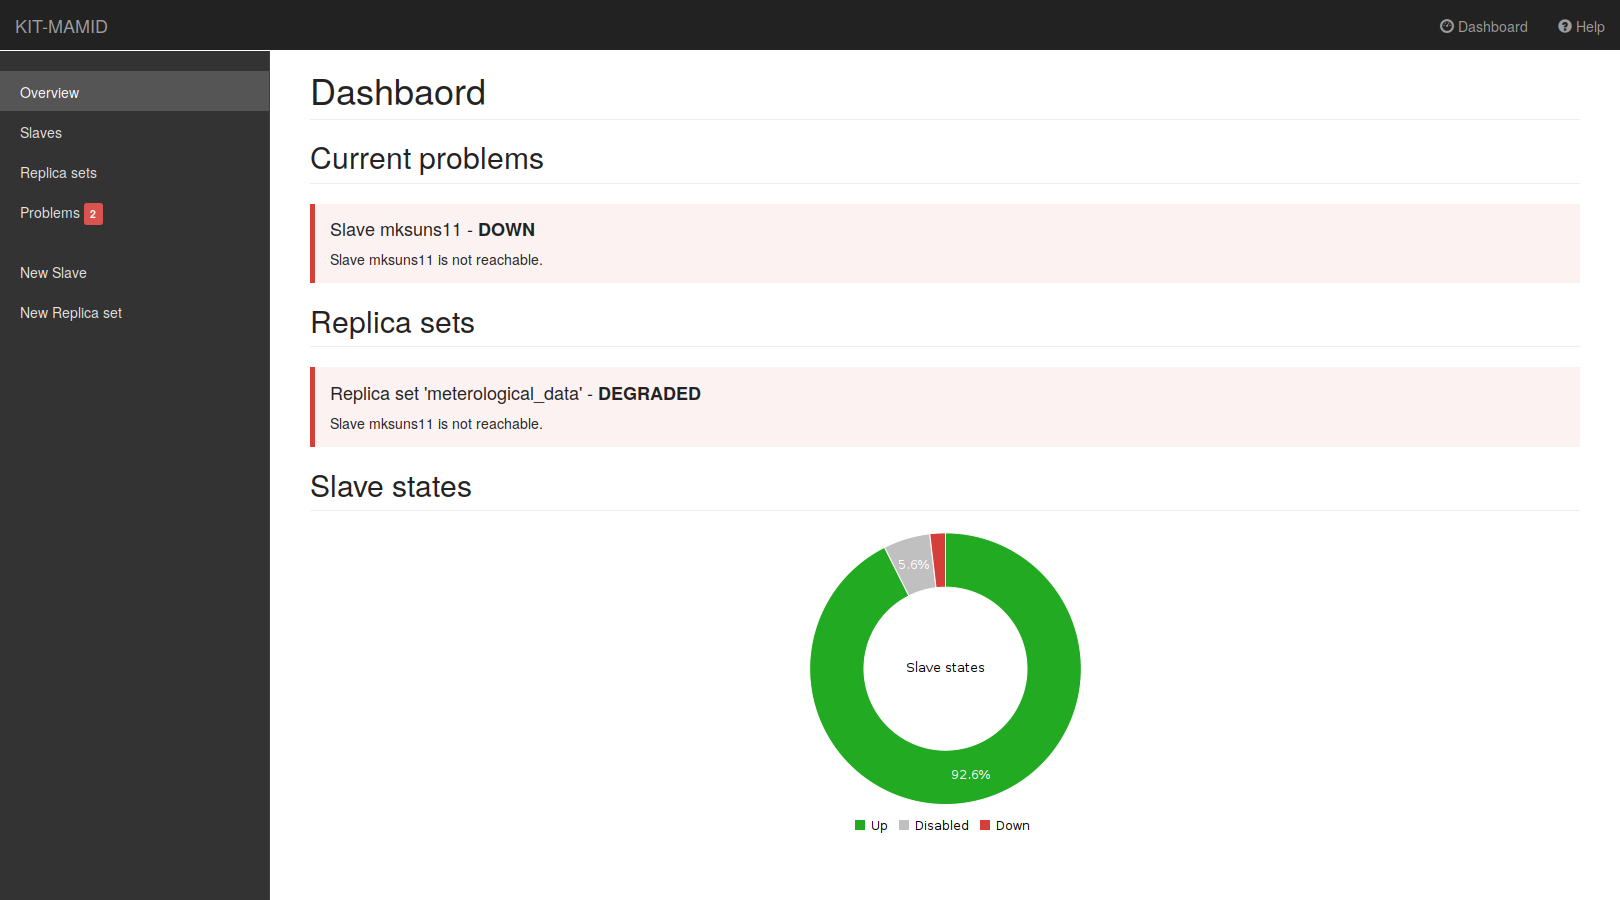
\includegraphics[width=\textwidth]{screenshots/dashboard}
	\caption{The overview view}
\end{figure}
\begin{figure}[H]
	\centering
	\includegraphics[width=\textwidth]{screenshots/slaves}
	\caption{The slaves view}
\end{figure}
\begin{figure}[H]
	\centering
	\includegraphics[width=\textwidth]{screenshots/replica_sets}
	\caption{The replica sets view}
\end{figure}
\begin{figure}[H]
	\centering
	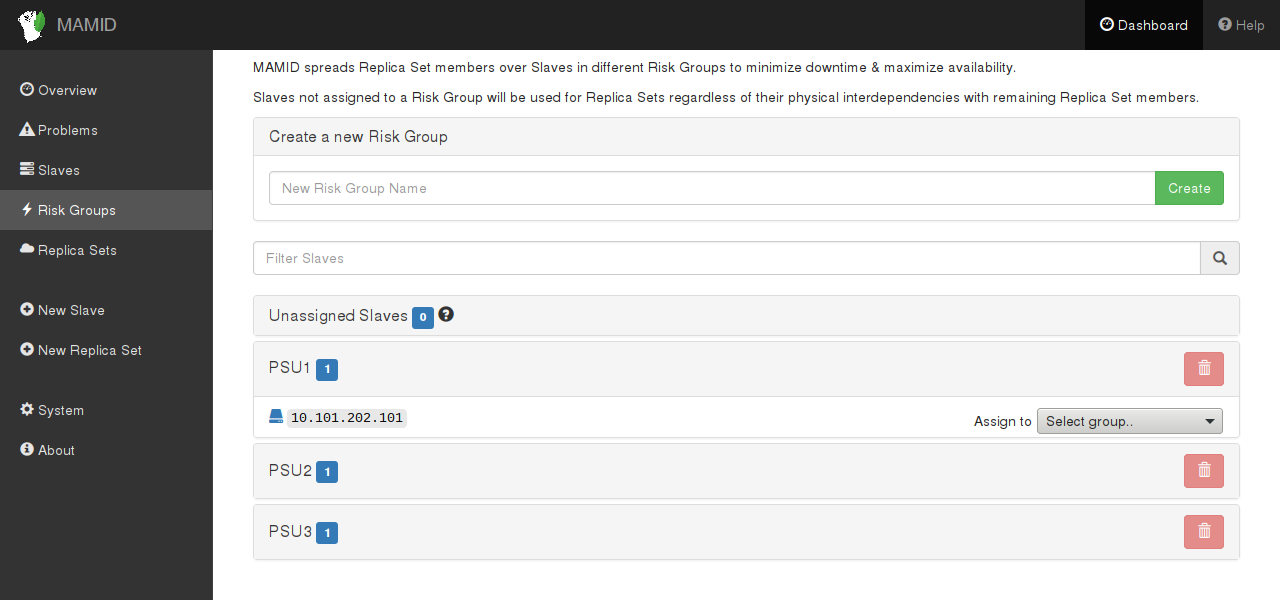
\includegraphics[width=\textwidth]{screenshots/risk_groups}
	\caption{The risk groups view}
\end{figure}
\begin{figure}[H]
	\centering
	\includegraphics[width=\textwidth]{screenshots/problems}
	\caption{The problems view}
\end{figure}
\begin{figure}[H]
	\centering
	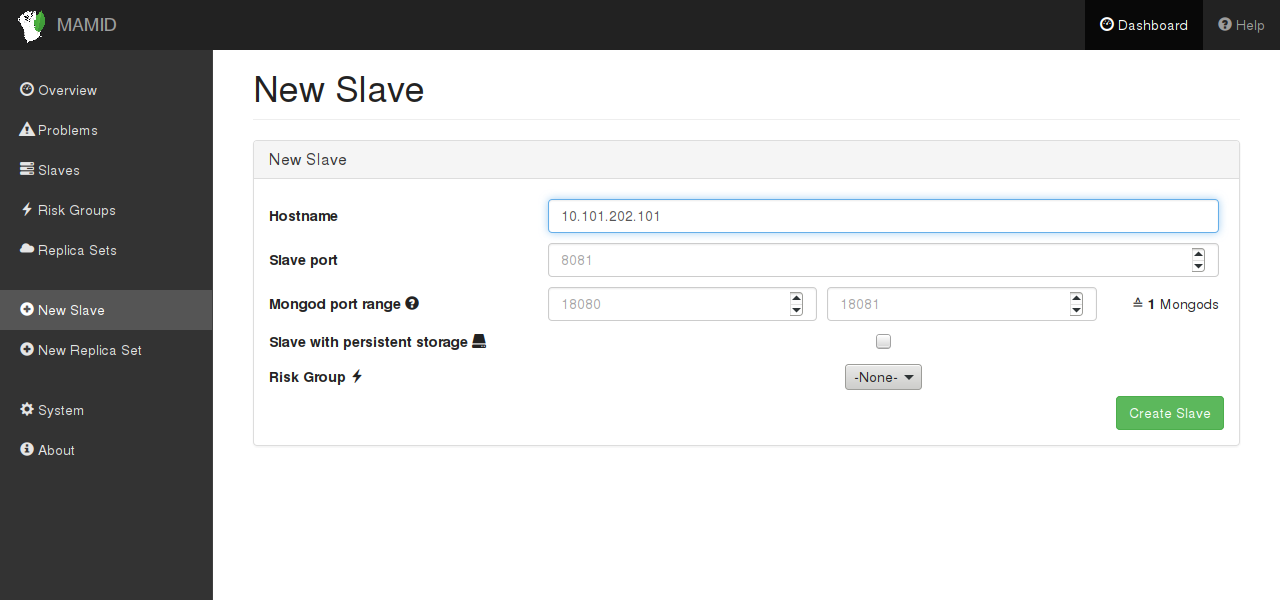
\includegraphics[width=\textwidth]{screenshots/new_slave}
	\caption{The new slave wizard}
\end{figure}
\begin{figure}[H]
	\centering
	\includegraphics[width=\textwidth]{screenshots/new_replica_set}
	\caption{The new replica set wizard}
\end{figure}
\subsection{Modifying a slave}
\begin{figure}[H]
	\centering
	\includegraphics[width=\textwidth]{screenshots/slave_edit_active.png}
	\caption{The slave edit view with a slave in 'active' state}
\end{figure}
\begin{figure}[H]
	\centering
	\includegraphics[width=\textwidth]{screenshots/slave_edit_unknown.png}
	\caption{The slave edit view with a slave in 'unknown' state}
\end{figure}
\begin{figure}[H]
	\centering
	\includegraphics[width=\textwidth]{screenshots/slave_edit_disabled.png}
	\caption{The slave edit view with a slave in 'disabled' state}
\end{figure}
\begin{figure}[H]
	\centering
	\includegraphics[width=\textwidth]{screenshots/slave_edit_maintenance}
	\caption{The slave edit view with a slave in 'maintenance mode'}
\end{figure}
\begin{figure}[H]
	\centering
	\includegraphics[width=\textwidth]{screenshots/slave_remove}
	\caption{Removing a slave}
\end{figure}

\subsection{Modifying a replica set}
\begin{figure}[H]
	\centering
	\includegraphics[width=\textwidth]{screenshots/replica_set_overview_active.png}
	\caption{The replica set overview with a normal operating replica set}
\end{figure}
\begin{figure}[H]
	\centering
	\includegraphics[width=\textwidth]{screenshots/replica_set_overview_degraded}
	\caption{The replica set overview with a degraded replica set}
\end{figure}
\begin{figure}[H]
	\centering
	\includegraphics[width=\textwidth]{screenshots/replica_set_remove}
	\caption{Removing a replica set}
\end{figure}
%Form:
%Name [: Beschreibung]
%Beschreibung: satz ohne subjekt, also klein und ohne Punkt; Strichpunkt getrennt

%\begin{enumerate}
%\item
%\end{enumerate}

%text...

\section{Test Cases and Scenarios}
% Vorbedinung, Aktionen, Nachbedingung 
\subsection{Test Cases}
Bei allen Testfällen gilt als Vorbedingung, dass \mamid gestartet ist (außer es ist explizit gefordert, dass es gestoppt ist).
\begin{description}
\itemsep 1em
\subsubsection{Kernfunktionen}
\oitem{TF}{testen} a testcase.
\testfall[\ref{WK:beschlArc}] %testet:
    {foo} %vorbedingung
    {bar} % ablauf
    {jon} % erwa. ergebnis
\end{description}
\subsection{Scenarios}
% all. vorbed.
Unless explicitly stated, the \acrshort{gui}'s home page is always opened in the tester's browser. %TODO ref home page

\begin{description}

\oitem{TS}{} Adding Machines to the Cluster
\testsequence
[\ref{F:gui_crud_inventory}, \ref{F:master_api_crud_slaves}, \ref{F:gui_set_slave_mode}, \ref{F:master_api_set_slave_mode}, \ref{F:master_inventory_persist_conf_state}]
{
	A machine $M$ with installed \gls{slave} software is connected to the \gls{cluster} network. The \gls{administrator} configures that the \gls{slave} software is started on boot.
}
{
	\begin{itemize}
		\item The \gls{administrator} navigates to the 'slave management section' in the \hyperref[SM:GUI]{GUI}.
		\item The \gls{administrator} adds the slave $S$ on $M$ using the 'add slave form'. %TODO ref testseq and ui
		\item The \gls{administrator} sets $S$ from \gls{disabled mode} to \gls{active mode}.
	\end{itemize}
}

\oitem{TS}{} Removing Machines from the Cluster
\testsequence
[\ref{F:gui_crud_inventory}, \ref{F:master_api_crud_slaves}, \ref{F:gui_set_slave_mode}, \ref{F:master_api_set_slave_mode}, \ref{F:master_inventory_persist_conf_state}, \ref{F:layout_cluster_config}, \ref{F:master_alloc_communicate_config}]
{
	A machine $M$ with installed \gls{slave} software shall be removed from the cluster.
}
{
	\begin{itemize}
		\item The \gls{administrator} navigates to the 'slave management section' in the \hyperref[SM:GUI]{GUI}.
		\item The \gls{administrator} selects the \gls{slave} $S$ and sets it to \gls{disabled mode}. %TODO ref testseq and ui
		\item The \hyperref[SM:Master]{master} determines a new \gls{cluster} layout to repair $S$'s former \glspl{replica set}.
		\item The \hyperref[SM:Master]{master} communicates the desired configuration to the appropriate \glspl{slave}.
		\item The \hyperref[SM:GUI]{GUI} now allows the \gls{administrator} to delete $S$ from the \gls{inventory}.
		\item The \gls{administrator} deletes $S$ from the \gls{inventory}. %TODO ref testseq and ui
		\item The \gls{administrator} can now physically remove $M$ from the \gls{cluster}.
	\end{itemize}
}


\oitem{TS}{} Temporarily Unreachable Slave
\testsequence
[\ref{F:master_monitor_config}, \ref{F:master_api_error_reports}, \ref{F:gui_display_errors}, \ref{F:gui_set_slave_mode}, \ref{F:msp_trans_reachability}]
{
	A \gls{slave} $S$ becomes unreachable because of broken network cable.
}
{
	\begin{itemize}
		\item \hyperref[SM:NotificationManager]{NotificationManager} sends an e-mail notification to the \gls{administrator}.
		\item \glslink{administrator}{Administrator} responds to the e-mail notification by opening the 'error reports' section in the web interface. %TODO ref
		\item \hyperref[SM:GUI]{GUI} offers to set $S$ into \glslink{maintenance mode}{maintenance} or \gls{disabled mode}.
		\item \glslink{administrator}{Administrator} does not choose either of the options but replaces the broken cable.
		\item \hyperref[SM:Master]{Master} reaches $S$ again.
		\item \hyperref[SM:Master]{Master} determines that configuration is still as expected.
		\item \hyperref[SM:Master]{Master} removes $S$ from the error report.
	\end{itemize}
}


\oitem{TS}{} Defective Slave
\testsequence
[\ref{F:master_monitor_config}, \ref{F:master_api_error_reports}, \ref{F:gui_display_errors}, \ref{F:gui_set_slave_mode}, \ref{F:master_api_set_slave_mode}, \ref{F:master_inventory_persist_conf_state}, \ref{F:layout_cluster_config}, \ref{F:master_alloc_resp_pv_counts}, \ref{F:master_alloc_resp_mode}, \ref{F:master_alloc_communicate_config}, \ref{F:slave_control_procs}, \ref{F:slave_enforce_config}, \ref{F:slave_report_config}, \ref{F:msp_trans_config}, \ref{F:msp_trans_reachability}, \ref{F:master_monitor_config}]
{
	A \gls{slave} $S$ becomes permanently unreachable because there was a short-circuit on its mainboard which needs to be replaced. The admin has no spare mainboards left and has to wait for replacement hardware to arrive. However, there is at least one \glslink{active mode}{active} \gls{slave} allowed to take over the role of the failed one.
}
{
	\begin{itemize}
		\item After $S$ becomes unavailable the \hyperref[SM:NotificationManager]{NotificationManager} sends an e-mail notification to the \gls{administrator}.
		\item \glslink{administrator}{Administrator} responds to e-mail notification by opening the 'error reports' section in web interface %TODO ref
		\item \hyperref[SM:GUI]{GUI} offers to set $S$ into \glslink{maintenance mode}{maintenance} or \gls{disabled mode}.
		\item \glslink{administrator}{Administrator} chooses \gls{disabled mode}.
		\item \hyperref[SM:Master]{Master} selects a \gls{slave} $S'$ as a replacement for $S$ and communicates the appropriate configuration to $S'$
		\item $S'$ starts a new \gls{MongoDB} process and enforces the received configuration.
		\item $S'$ reports successful configuration to \hyperref[SM:Master]{master}.
		\item \hyperref[SM:Master]{Master} removes $S$ from the error report.
	\end{itemize}
}


\oitem{TS}{} System Maintenance
\testsequence
[\ref{F:gui_crud_inventory}, \ref{F:master_api_crud_slaves}, \ref{F:gui_set_slave_mode}, \ref{F:master_api_set_slave_mode}, \ref{F:master_inventory_persist_conf_state}, \ref{F:master_alloc_communicate_config}, \ref{F:slave_control_procs}, \ref{F:slave_enforce_config}, \ref{F:slave_report_config}, \ref{F:msp_trans_config}]
{
	A \gls{slave} $S$ needs to be rebooted to install security updates to the installed software.
}
{
	\begin{itemize}
		\item The \gls{administrator} navigates to the 'slave management section' in the \hyperref[SM:GUI]{GUI}. %TODO ui ref
		\item The \gls{administrator} selects $S$ and sets it to \gls{maintenance mode}.
		\item The \gls{administrator} installs the security updates and reboots the machine (killing the \gls{slave} instance and all its \gls{MongoDB} instances).
		\item The \gls{slave} process $S$ is restarted by the system's service manager after reboot.
		\item The \gls{administrator} sets $S$ back to \gls{active mode}.
		\item The \hyperref[SM:Master]{master} communicates the desired configuration to $S$.
		\item $S$ starts the \gls{MongoDB} processes and configures \gls{replica set} membership if required by the communicated configuration.
	\end{itemize}
}


\oitem{TS}{} Adding a Replica Set
\testsequence
[\ref{F:gui_crud_replica_sets}, \ref{F:master_api_crud_repl_set_config}, \ref{F:layout_cluster_config}, \ref{F:master_alloc_resp_pv_counts}, \ref{F:master_alloc_resp_mode}, \ref{F:master_alloc_communicate_config}, \ref{F:slave_control_procs}, \ref{F:slave_enforce_config}, \ref{F:msp_trans_config}]
{
	The \gls{administrator} wants to add a \gls{replica set} with $p \in \mathbb{N}$ \glslink{persistent storage}{persistent} members and $v \in \mathbb{N}$ \glslink{volatile storage}{volatile} members. $(p+v) >= 3 \land (p+v) is odd$. Enough \glspl{slave} with sufficient free \gls{MongoDB} \hyperref[D:slave_mongod_portrange]{ports} are available.
}
{
	\begin{itemize}
		\item The \gls{administrator} navigates to 'replica set management section'. %TODO ref ui
		\item The \gls{administrator} adds a new replica set $R$ using the 'add replica set form' with constraints $p$ and $v$. %TODO ref ui and testsequence
		\item The \hyperref[SM:Master]{master} finds appropriate \glspl{slave} for hosting members of $R$ (\hyperref[SM:master_clusterallocator]{Master::ClusterAllocator}).
		\item The \hyperref[SM:Master]{master} communicates the desired configuration to the appropriate \glspl{slave} $Z$.
		\item The \glspl{slave} in $Z$ apply the received configuration.
	\end{itemize}
}

\oitem{TS}{} Destroying a Replica Set
\testsequence
[\ref{F:gui_crud_replica_sets}, \ref{F:master_api_crud_repl_set_config}, \ref{F:layout_cluster_config}, \ref{F:master_alloc_resp_pv_counts}, \ref{F:master_alloc_resp_mode}, \ref{F:master_alloc_communicate_config}, \ref{F:slave_control_procs}, \ref{F:slave_enforce_config}, \ref{F:msp_trans_config}]
{
	The \gls{administrator} wants to destroy a \gls{replica set} $R$.
}
{
	\begin{itemize}
		\item The \gls{administrator} navigates to 'replica set management section'. %TODO ref ui
		\item The \gls{administrator} selects $R$ and clicks the remove button. % TODO ref testseq and ui
		\item The \hyperref[SM:GUI]{GUI} prompts the \gls{administrator} for confirmation.
		\item The \gls{administrator} confirms the removal.
		\item The \hyperref[SM:Master]{master} persists the change and communicates to the \glspl{slave} that \gls{host} members of $R$ must kill the respective \gls{MongoDB} processes.
		\item The \glspl{slave} apply the received instructions.
	\end{itemize}
}

\end{description}


\newpage
\glsaddallunused
\makeatletter
\newglossarystyle{myAltlist}{
  \glossarystyle{altlist} % base this style on altlist
  \renewcommand*{\glossaryentryfield}[5]{
  \item[\glsentryitem{##1}\glstarget{##1}{##2}]
    \mbox{}\par\nobreak\@afterheading
    ##3\glspostdescription\space On page ##5.
  }
}
\makeatother
\glsaddall
\printglossary[type=main, title={Glossary}, toctitle={Glossary}, style=myAltlist]

\end{document}
